\newif\ifglobal

%%%%%%%%%%%%%%%%%%%%%%%
%%% Compile to view %%%
%%%%%%%%%%%%%%%%%%%%%%%

%%%%%%%%%%%%%%%%%%%%%%%%%%%%%%%%%%%%%%%%%%%%%%%%%%%
%%% Readme:                                     %%%
%%% https://www.overleaf.com/read/bwdjvfjksvjy/ %%%
%%%%%%%%%%%%%%%%%%%%%%%%%%%%%%%%%%%%%%%%%%%%%%%%%%%

% >>> M?: marks a module setting number or important notice

% >>> M4: Set {./relative-path} to external files for this module <<<
\def \modulefiles {./22-INTMTRX}
% To add an external file, use:
% (Replace '---' with actual filename)
% '\input{\modulefiles/tables/---.tex}' for tables
% '\includegraphics{\modulefiles/figures/---}' for figures
% '\subfile{\modulefiles/---}' for register files

% >>> M1: This module is in global project? <<<
% 'YES' - uncomment; 'NO' - comment out
\globaltrue

\ifglobal
    \documentclass[main\_\_CN.tex]{subfiles}

\else
    % Font "FandolSong-Regular" used by ctex does not have GSUB table.
    % It causes warnings that do not affect compilation and can be ignored.
    \PassOptionsToPackage{quiet}{fontspec}

    \documentclass[openany, 10pt]{book}

    % >>> M2: In ./00-shared/preamble-trm-module, also find
    %         settings for visibility of todo notes, watermark <<<
    \usepackage{preamble-trm-module}


    % Enable Chinese typesetting
    \usepackage{ctex}

    % >>> M3: Temporary labels in Chinese
    %         you can add your own labels there <<<
    \myexternaldocument{./00-shared/temp-labels-cn}

\fi %\ifglobal


\setcounter{secnumdepth}{4}

% >>> M5: If this module needs any updates in
% './00-shared/preamble-trm-module.sty'
% (include additional package, etc.), contact your module PM
% or create the file './00-shared/changelog.tex' make the
% necessary updates yourself and document them in this file <<<


\begin{document}


% Sets language into which pre-defined bits of text are translated
\selectlanguage{chinese}

% Do not delete this block
\ifglobal
% Add the following front matter if
% this module is outside of global project
\else
    \InputIfFileExists{readme}{}{}
    {\let\clearpage\relax \listoftodos}
    \tableofcontents
    %\listoftables
    %\listoffigures
\fi


%%%%%%%%%%%%%%%%%%%%%%%%%
%%% TRM Module Begins %%%
%%%%%%%%%%%%%%%%%%%%%%%%%

\hypertarget{intmtrx}{}
\chapter{中断矩阵 (INTERRUPT)}
\label{mod:intmtrx}


\section{概述}

\chipname{} 中断矩阵将任一外部中断源单独分配到双核 CPU 的任一外部中断上，以便在外设中断信号产生后，及时通知 CPU0 或 CPU1 进行处理。

外部中断源必须经中断矩阵分配至 CPU0/CPU1 外部中断，主要是因为：
\begin{itemize}
    \item \chipname{} 有 99 个外部中断源，但每个 CPU 只有 32 个中断。将这些外部中断源映射至 CPU0 中断或 CPU1 中断需要使用中断矩阵。
    \item 通过中断矩阵，可以根据应用需要，将一个外部中断源映射至多个 CPU0 中断或 CPU1 中断。
\end{itemize}

\section{主要特性}

\begin{itemize}
    \item 接收 99 个外部中断源作为输入
    \item 生成 26 个 CPU0 的外部中断和 26 个 CPU1 的外部中断作为输出。

    注意，CPU0 剩余的 6 个中断和 CPU1 剩余的 6 个中断均为内部中断
    \item 支持屏蔽 CPU 的 NMI 类型中断
    \item 支持查询外部中断源当前的中断状态
\end{itemize}

中断矩阵的结构如图 \ref{fig:interrupt-matrix-structure} 所示。

\begin{figure}[h!]
    \centering
    {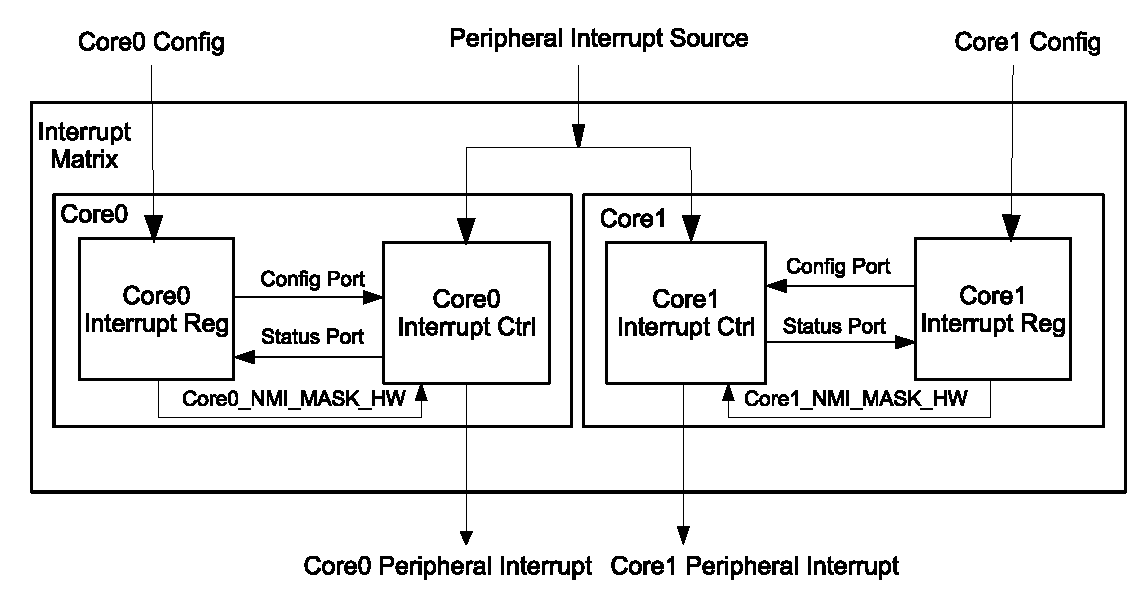
\includegraphics[width=0.9\textwidth]{22-INTMTRX/figures/22-INTMTRX-struct.eps}}
    \caption{中断矩阵结构图}
    \label{fig:interrupt-matrix-structure}
\end{figure}

所有外部中断源产生的中断信号均可由 CPU0 或 CPU1 进行处理。配置 \hyperref[CPU0RegisterSummary]{CPU0 中断寄存器}（图 \ref{fig:interrupt-matrix-structure} Core0 Interrupt Reg 模块）可将外部中断源分配给 CPU0 的外部中断，此时外部中断源产生的中断信号会由 CPU0 响应处理。同理配置 \hyperref[CPU1RegisterSummary]{CPU1 中断寄存器}（图 \ref{fig:interrupt-matrix-structure} Core1 Interrupt Reg 模块）可将中断信号交由 CPU1 响应处理。也可将外部中断源同时分配给 CPU0 和 CPU1, 此时 CPU0 和 CPU1 都会接收到中断信号。

\section{功能描述}

\subsection{外部中断源}

\chipname{} 共有 99 个外部中断源。表 \ref{tab:peripheral-interrupt-config-status-source} 列出了所有外部中断源，以及对应的中断配置寄存器与中断状态寄存器。

\begin{itemize}
    \item ``No."：表示外部中断源序号，范围：0 \verb+~+ 98
    \item ``中断源"：表示所有外部中断源
    \item ``配置寄存器"：用于将外部中断源分配至 CPU0/CPU1 外部中断
    \item ``状态寄存器"：用于读取中断源的中断状态
    \begin{itemize}
        \item ``状态寄存器 - 位"：表示在状态寄存器中的比特位置
        \item ``状态寄存器 - 名称"：表示状态寄存器的名称
    \end{itemize}

\end{itemize}

中断源与同一行中断配置寄存器和中断状态寄存器位一一对应，例如：中断源 MAC\_INTR 对应的中断配置寄存器为 \hyperref[regdesc:INTERRUPTCORE0MACINTRMAPREG]{INTERRUPT\_CORE\regindex{x}\_MAC\_INTR\_MAP\_REG}，
对应的中断状态寄存器位为 \hyperref[regdesc:INTERRUPTCORE0INTRSTATUS0REG]{INTERRUPT\_CORE\regindex{x}\_INTR\_STATUS\\\_0\_REG} 的 0 比特。

注意，表格中 CORE\regindex{x} 可以是 CORE0 (CPU0) 或 CORE1 (CPU1)。
\clearpage
\begin{landscape}

\begin{footnotesize}
\begin{longtable}[c]{|*{5}{c|}}
    \caption{CPU 外部中断配置寄存器、外部中断状态寄存器、外部中断源}
    \label{tab:peripheral-interrupt-config-status-source}\\
    
    \hline
    \rowcolor{gray!25}
    & & & \multicolumn{2}{c|}{\textbf{状态寄存器}} \\
    \cline{4-5}
    \rowcolor{gray!25}
    \multirow{-2}*{\textbf{No.}} & \multirow{-2}*{\textbf{中断源}} & \multirow{-2}*{\textbf{配置寄存器}} & \textbf{位} & \textbf{名称} \\
    \hline
    \endfirsthead
    
    \hline
    \rowcolor{gray!25}
    & & & \multicolumn{2}{c|}{\textbf{状态寄存器}} \\
    \cline{4-5}
    \rowcolor{gray!25}
    \multirow{-2}*{\textbf{No.}} & \multirow{-2}*{\textbf{中断源}} & \multirow{-2}*{\textbf{配置寄存器}} & \textbf{位} & \textbf{名称} \\
    \hline
    \endhead
    \endfoot
    

		0 & MAC\_INTR & \hyperref[regdesc:INTERRUPTCORE0MACINTRMAPREG]{INTERRUPT\_CORE\regindex{x}\_MAC\_INTR\_MAP\_REG} & 0 & \multirow{32}*{\makecell{\hyperref[regdesc:INTERRUPTCORE0INTRSTATUS0REG]{INTERRUPT\_CORE\regindex{x}\_INTR\_STATUS\_0\_REG}}}                        	\\
    \cline{1-4}                                           
    1 & MAC\_NMI & \hyperref[regdesc:INTERRUPTCORE0CACHECORE1ACSINTMAPREG]{INTERRUPT\_CORE\regindex{x}\_MAC\_NMI\_MAP\_REG} & 1 & \\
    \cline{1-4}                                           
    2 & PWR\_INTR & \hyperref[regdesc:INTERRUPTCORE0CACHECORE1ACSINTMAPREG]{INTERRUPT\_CORE\regindex{x}\_PWR\_INTR\_MAP\_REG} & 2 &                           	\\
    \cline{1-4}  
    3 & BB\_INT & \hyperref[regdesc:INTERRUPTCORE0CACHECORE1ACSINTMAPREG]{INTERRUPT\_CORE\regindex{x}\_BB\_INT\_MAP\_REG} & 3 &                          	\\
    \cline{1-4}
    4 & BT\_MAC\_INT & \hyperref[regdesc:INTERRUPTCORE0CACHECORE1ACSINTMAPREG]{INTERRUPT\_CORE\regindex{x}\_BT\_MAC\_INT\_MAP\_REG} & 4 &                          	\\
    \cline{1-4}
    5 & BT\_BB\_INT & \hyperref[regdesc:INTERRUPTCORE0CACHECORE1ACSINTMAPREG]{INTERRUPT\_CORE\regindex{x}\_BT\_BB\_INT\_MAP\_REG} & 5 &                          	\\
    \cline{1-4}
    6 & BT\_BB\_NMI  & \hyperref[regdesc:INTERRUPTCORE0CACHECORE1ACSINTMAPREG]{INTERRUPT\_CORE\regindex{x}\_BT\_BB\_NMI\_MAP\_REG} & 6 &                          	\\
    \cline{1-4}
    7 & RWBT\_IRQ & \hyperref[regdesc:INTERRUPTCORE0CACHECORE1ACSINTMAPREG]{INTERRUPT\_CORE\regindex{x}\_RWBT\_IRQ\_MAP\_REG} & 7 &                          	\\
    \cline{1-4}
    8 & RWBLE\_IRQ & \hyperref[regdesc:INTERRUPTCORE0CACHECORE1ACSINTMAPREG]{INTERRUPT\_CORE\regindex{x}\_RWBLE\_IRQ\_MAP\_REG} & 8 &                          	\\
    \cline{1-4}
    9 & RWBT\_NMI & \hyperref[regdesc:INTERRUPTCORE0CACHECORE1ACSINTMAPREG]{INTERRUPT\_CORE\regindex{x}\_RWBT\_NMI\_MAP\_REG} & 9 &                          	\\
    \cline{1-4}
    10 & RWBLE\_NMI & \hyperref[regdesc:INTERRUPTCORE0CACHECORE1ACSINTMAPREG]{INTERRUPT\_CORE\regindex{x}\_RWBLE\_NMI\_MAP\_REG} & 10 &                          	\\
    \cline{1-4}
    11 & I2C\_MST\_INT & \hyperref[regdesc:INTERRUPTCORE0CACHECORE1ACSINTMAPREG]{INTERRUPT\_CORE\regindex{x}\_I2C\_MST\_INT\_MAP\_REG} & 11 &                          	\\
    \cline{1-4}
    12 & 保留 & 保留 & 12 &                          	\\
    \cline{1-4}
    
    13 & 保留 & 保留 & 13 &                          	\\
    \cline{1-4}
    14 & UHCI0\_INTR & \hyperref[regdesc:INTERRUPTCORE0CACHECORE1ACSINTMAPREG]{INTERRUPT\_CORE\regindex{x}\_UHCI0\_INTR\_MAP\_REG} & 14 &                          	\\
    \cline{1-4}
    15 & 保留 & 保留 & 15 &                          	\\
    \cline{1-4}
    16 & GPIO\_INTERRUPT\_CPU & \hyperref[regdesc:INTERRUPTCORE0CACHECORE1ACSINTMAPREG]{INTERRUPT\_CORE\regindex{x}\_GPIO\_INTERRUPT\_CPU\_MAP\_REG} & 16 &                          	\\
    \cline{1-4}
    17 & GPIO\_INTERRUPT\_CPU\_NMI & \hyperref[regdesc:INTERRUPTCORE0CACHECORE1ACSINTMAPREG]{INTERRUPT\_CORE\regindex{x}\_GPIO\_INTERRUPT\_CPU\_NMI\_MAP\_REG} & 17 &                          	\\
    \cline{1-4}
    18 & 保留 & 保留 & 18 &                          	\\
    \cline{1-4}
    19 & 保留 & 保留 & 19 &                          	\\
    \cline{1-4}
    20 & SPI\_INTR\_1 & \hyperref[regdesc:INTERRUPTCORE0CACHECORE1ACSINTMAPREG]{INTERRUPT\_CORE\regindex{x}\_SPI\_INTR\_1\_MAP\_REG} & 20 &                          	\\
    \cline{1-4}
    21 & SPI\_INTR\_2 & \hyperref[regdesc:INTERRUPTCORE0CACHECORE1ACSINTMAPREG]{INTERRUPT\_CORE\regindex{x}\_SPI\_INTR\_2\_MAP\_REG} & 21 &                          	\\
    \cline{1-4}
    22 & SPI\_INTR\_3 & \hyperref[regdesc:INTERRUPTCORE0CACHECORE1ACSINTMAPREG]{INTERRUPT\_CORE\regindex{x}\_SPI\_INTR\_3\_MAP\_REG} & 22 &                          	\\
    \cline{1-4}
    23 & 保留 & 保留 & 23 &                          	\\
    \cline{1-4}
    24 & LCD\_CAM\_INT & \hyperref[regdesc:INTERRUPTCORE0CACHECORE1ACSINTMAPREG]{INTERRUPT\_CORE\regindex{x}\_LCD\_CAM\_INT\_MAP\_REG} & 24 &                          	\\
    \cline{1-4}
    25 & I2S0\_INT & \hyperref[regdesc:INTERRUPTCORE0CACHECORE1ACSINTMAPREG]{INTERRUPT\_CORE\regindex{x}\_I2S0\_INT\_MAP\_REG} & 25 &                          	\\
    \cline{1-4}
    26 & I2S1\_INT & \hyperref[regdesc:INTERRUPTCORE0CACHECORE1ACSINTMAPREG]{INTERRUPT\_CORE\regindex{x}\_I2S1\_INT\_MAP\_REG} & 26 &                          	\\
    \cline{1-4}
    27 & UART\_INTR & \hyperref[regdesc:INTERRUPTCORE0CACHECORE1ACSINTMAPREG]{INTERRUPT\_CORE\regindex{x}\_UART\_INTR\_MAP\_REG} & 27 &                          	\\
    \cline{1-4}
    28 & UART1\_INTR & \hyperref[regdesc:INTERRUPTCORE0CACHECORE1ACSINTMAPREG]{INTERRUPT\_CORE\regindex{x}\_UART1\_INTR\_MAP\_REG} & 28 &                          	\\
    \cline{1-4}
    29 & UART2\_INTR & \hyperref[regdesc:INTERRUPTCORE0CACHECORE1ACSINTMAPREG]{INTERRUPT\_CORE\regindex{x}\_UART2\_INTR\_MAP\_REG} & 29 &                          	\\
    \cline{1-4}
    30 & SDIO\_HOST\_INTERRUPT & \hyperref[regdesc:INTERRUPTCORE0CACHECORE1ACSINTMAPREG]{INTERRUPT\_CORE\regindex{x}\_SDIO\_HOST\_INTERRUPT\_MAP\_REG} & 30 &                          	\\
    \cline{1-4}
    31 & PWM0\_INTR & \hyperref[regdesc:INTERRUPTCORE0CACHECORE1ACSINTMAPREG]{INTERRUPT\_CORE\regindex{x}\_PWM0\_INTR\_MAP\_REG} & 31 &                          	\\
    \hline
    
    
    32 & PWM1\_INTR & \hyperref[regdesc:INTERRUPTCORE0CACHECORE1ACSINTMAPREG]{INTERRUPT\_CORE\regindex{x}\_PWM1\_INTR\_MAP\_REG} & 0 &  \multirow{3}*{\makecell{\hyperref[regdesc:INTERRUPTCORE0INTRSTATUS1REG]{INTERRUPT\_CORE\regindex{x}\_INTR\_STATUS\_1\_REG}}}                    	
    \\
    \cline{1-4}                                           
    33 & 保留 & 保留 & 1 &                          	\\
    \cline{1-4}
    34  & 保留 & 保留  & 2 &                          	\\
    \hline
    
    35  & LEDC\_INT  & \hyperref[regdesc:INTERRUPTCORE0CACHECORE1ACSINTMAPREG]{INTERRUPT\_CORE\regindex{x}\_LEDC\_INT\_MAP\_REG} & 3 &                          	\\
    \cline{1-4}
    36  & EFUSE\_INT  & \hyperref[regdesc:INTERRUPTCORE0CACHECORE1ACSINTMAPREG]{INTERRUPT\_CORE\regindex{x}\_EFUSE\_INT\_MAP\_REG} & 4 &                          	\\
    \cline{1-4}
    37  & TWAI\_INT & \hyperref[regdesc:INTERRUPTCORE0CACHECORE1ACSINTMAPREG]{INTERRUPT\_CORE\regindex{x}\_TWAI\_INT\_MAP\_REG} & 5 &                          	\\
    \cline{1-4} 
    38  & USB\_INTR  & \hyperref[regdesc:INTERRUPTCORE0CACHECORE1ACSINTMAPREG]{INTERRUPT\_CORE\regindex{x}\_USB\_INTR\_MAP\_REG}  & 6 &                          	\\
    \cline{1-4}
    
    39 & RTC\_CORE\_INTR &\hyperref[regdesc:INTERRUPTCORE0CACHECORE1ACSINTMAPREG]{INTERRUPT\_CORE\regindex{x}\_RTC\_CORE\_INTR\_MAP\_REG} & 7 & \multirow{25}*{\makecell{\hyperref[regdesc:INTERRUPTCORE0INTRSTATUS1REG]{INTERRUPT\_CORE\regindex{x}\_INTR\_STATUS\_1\_REG}}}                        	\\
    \cline{1-4}
 
    40  & RMT\_INTR & \hyperref[regdesc:INTERRUPTCORE0CACHECORE1ACSINTMAPREG]{INTERRUPT\_CORE\regindex{x}\_RMT\_INTR\_MAP\_REG} &8  &                          	\\
    \cline{1-4}
    41  & PCNT\_INTR  & \hyperref[regdesc:INTERRUPTCORE0CACHECORE1ACSINTMAPREG]{INTERRUPT\_CORE\regindex{x}\_PCNT\_INTR\_MAP\_REG} & 9  &                          	\\
    \cline{1-4}
    42  & I2C\_EXT0\_INTR  & \hyperref[regdesc:INTERRUPTCORE0CACHECORE1ACSINTMAPREG]{INTERRUPT\_CORE\regindex{x}\_I2C\_EXT0\_INTR\_MAP\_REG}  &10  &                          	\\
    \cline{1-4}
    43  & I2C\_EXT1\_INTR & \hyperref[regdesc:INTERRUPTCORE0CACHECORE1ACSINTMAPREG]{INTERRUPT\_CORE\regindex{x}\_I2C\_EXT1\_INTR\_MAP\_REG}  &11  &                          	\\
    \cline{1-4}
    44   & 保留 & 保留  &12  &                          	\\
    \cline{1-4}
    45   & 保留 & 保留  &13  &                          	\\
    \cline{1-4}
    46   & 保留 & 保留  &14  &                          	\\
    \cline{1-4}
    47   & 保留 & 保留  &15  &                          	\\
    \cline{1-4}
    48   & 保留 & 保留  &16  &                          	\\
    \cline{1-4}
    49   & 保留 & 保留  &17  &                          	\\
    \cline{1-4}
    50   & TG\_T0\_INT & \hyperref[regdesc:INTERRUPTCORE0CACHECORE1ACSINTMAPREG]{INTERRUPT\_CORE\regindex{x}\_TG\_T0\_INT\_MAP\_REG}  &18  &                          	\\
    \cline{1-4}
    51   & TG\_T1\_INT & \hyperref[regdesc:INTERRUPTCORE0CACHECORE1ACSINTMAPREG]{INTERRUPT\_CORE\regindex{x}\_TG\_T1\_INT\_MAP\_REG}  &19  &                          	\\
    \cline{1-4}
    52   & TG\_WDT\_INT & \hyperref[regdesc:INTERRUPTCORE0CACHECORE1ACSINTMAPREG]{INTERRUPT\_CORE\regindex{x}\_TG\_WDT\_INT\_MAP\_REG}  &20  &                          	\\
    \cline{1-4}
    53   & TG1\_T0\_INT & \hyperref[regdesc:INTERRUPTCORE0CACHECORE1ACSINTMAPREG]{INTERRUPT\_CORE\regindex{x}\_TG1\_T0\_INT\_MAP\_REG}  &21  &                          	\\
    \cline{1-4}
    54   & TG1\_T1\_INT & \hyperref[regdesc:INTERRUPTCORE0CACHECORE1ACSINTMAPREG]{INTERRUPT\_CORE\regindex{x}\_TG1\_T1\_INT\_MAP\_REG } &22  &                          	\\
    \cline{1-4}
    55   & TG1\_WDT\_INT & \hyperref[regdesc:INTERRUPTCORE0CACHECORE1ACSINTMAPREG]{INTERRUPT\_CORE\regindex{x}\_TG1\_WDT\_INT\_MAP\_REG } &23  &                          	\\
    \cline{1-4}
    56   & CACHE\_IA\_INT & \hyperref[regdesc:INTERRUPTCORE0CACHECORE1ACSINTMAPREG]{INTERRUPT\_CORE\regindex{x}\_CACHE\_IA\_INT\_MAP\_REG } &24  &                          	\\
    \cline{1-4}
    57   & SYSTIMER\_TARGET0\_INT & \hyperref[regdesc:INTERRUPTCORE0CACHECORE1ACSINTMAPREG]{INTERRUPT\_CORE\regindex{x}\_SYSTIMER\_TARGET0\_INT\_MAP\_REG}  &25  &                          	\\
    \cline{1-4}
    58 & SYSTIMER\_TARGET1\_INT &\hyperref[regdesc:INTERRUPTCORE0CACHECORE1ACSINTMAPREG]{INTERRUPT\_CORE\regindex{x}\_SYSTIMER\_TARGET1\_INT\_MAP\_REG}  & 26 &                            	\\
    \cline{1-4}
    59   & SYSTIMER\_TARGET2\_INT &\hyperref[regdesc:INTERRUPTCORE0CACHECORE1ACSINTMAPREG]{INTERRUPT\_CORE\regindex{x}\_SYSTIMER\_TARGET2\_INT\_MAP\_REG } &27  &                          	\\
    \cline{1-4}
    60   & SPI\_MEM\_REJECT\_INTR & \hyperref[regdesc:INTERRUPTCORE0CACHECORE1ACSINTMAPREG]{INTERRUPT\_CORE\regindex{x}\_SPI\_MEM\_REJECT\_INTR\_MAP\_REG}  &28  &                          	\\
    \cline{1-4}
    61   & DCACHE\_PRELOAD\_INT &\hyperref[regdesc:INTERRUPTCORE0CACHECORE1ACSINTMAPREG]{INTERRUPT\_CORE\regindex{x}\_DCACHE\_PRELOAD\_INT\_MAP\_REG  }&29  &                          	\\
    \cline{1-4}
    62   & ICACHE\_PRELOAD\_INT & \hyperref[regdesc:INTERRUPTCORE0CACHECORE1ACSINTMAPREG]{INTERRUPT\_CORE\regindex{x}\_ICACHE\_PRELOAD\_INT\_MAP\_REG  }& 30 &                          	\\
    \cline{1-4}
    63   & DCACHE\_SYNC\_INT &\hyperref[regdesc:INTERRUPTCORE0CACHECORE1ACSINTMAPREG]{INTERRUPT\_CORE\regindex{x}\_DCACHE\_SYNC\_INT\_MAP\_REG } & 31 &                          	\\
    \hline
    
    64 & ICACHE\_SYNC\_INT &\hyperref[regdesc:INTERRUPTCORE0CACHECORE1ACSINTMAPREG]{INTERRUPT\_CORE\regindex{x}\_ICACHE\_SYNC\_INT\_MAP\_REG} & 0 & \multirow{8}*{\makecell{\hyperref[regdesc:INTERRUPTCORE0INTRSTATUS2REG]{INTERRUPT\_CORE\regindex{x}\_INTR\_STATUS\_2\_REG}}}                      	\\
    \cline{1-4}
    
    65 & APB\_ADC\_INT & \hyperref[regdesc:INTERRUPTCORE0CACHECORE1ACSINTMAPREG]{INTERRUPT\_CORE\regindex{X}\_APB\_ADC\_INT\_MAP\_REG } & 1  &                          	\\
    \cline{1-4}
    66 & DMA\_IN\_CH0\_INT  & \hyperref[regdesc:INTERRUPTCORE0CACHECORE1ACSINTMAPREG]{INTERRUPT\_CORE\regindex{X}\_DMA\_IN\_CH0\_INT\_MAP\_REG  }&2  &                          	\\
    \cline{1-4}
    67 & DMA\_IN\_CH1\_INT  & \hyperref[regdesc:INTERRUPTCORE0CACHECORE1ACSINTMAPREG]{INTERRUPT\_CORE\regindex{x}\_DMA\_IN\_CH1\_INT\_MAP\_REG } &3  &                          	\\
    \cline{1-4}
    68 & DMA\_IN\_CH2\_INT  & \hyperref[regdesc:INTERRUPTCORE0CACHECORE1ACSINTMAPREG]{INTERRUPT\_CORE\regindex{x}\_DMA\_IN\_CH2\_INT\_MAP\_REG  }&4  &                          	\\
    \cline{1-4}
    69 & DMA\_IN\_CH3\_INT  & \hyperref[regdesc:INTERRUPTCORE0CACHECORE1ACSINTMAPREG]{INTERRUPT\_CORE\regindex{x}\_DMA\_IN\_CH3\_INT\_MAP\_REG}  &5  &                          	\\
    \cline{1-4}
    70 & DMA\_IN\_CH4\_INT  & \hyperref[regdesc:INTERRUPTCORE0CACHECORE1ACSINTMAPREG]{INTERRUPT\_CORE\regindex{x}\_DMA\_IN\_CH4\_INT\_MAP\_REG } &6  &                          	\\
    \cline{1-4}
    71 & DMA\_OUT\_CH0\_INT  & \hyperref[regdesc:INTERRUPTCORE0CACHECORE1ACSINTMAPREG]{INTERRUPT\_CORE\regindex{X}\_DMA\_OUT\_CH0\_INT\_MAP\_REG  }&7  &                          	\\
    \hline
    
    72 & DMA\_OUT\_CH1\_INT  & \hyperref[regdesc:INTERRUPTCORE0CACHECORE1ACSINTMAPREG]{INTERRUPT\_CORE\regindex{x}\_DMA\_OUT\_CH1\_INT\_MAP\_REG } &8  &   \multirow{24}*{\makecell{\hyperref[regdesc:INTERRUPTCORE0INTRSTATUS2REG]{INTERRUPT\_CORE\regindex{x}\_INTR\_STATUS\_2\_REG}}}                       	\\
    \cline{1-4}
    73 & DMA\_OUT\_CH2\_INT  & \hyperref[regdesc:INTERRUPTCORE0CACHECORE1ACSINTMAPREG]{INTERRUPT\_CORE\regindex{x}\_DMA\_OUT\_CH2\_INT\_MAP\_REG  }&9  &                          	\\
    \cline{1-4}
    74 & DMA\_OUT\_CH3\_INT  & \hyperref[regdesc:INTERRUPTCORE0CACHECORE1ACSINTMAPREG]{INTERRUPT\_CORE\regindex{x}\_DMA\_OUT\_CH3\_INT\_MAP\_REG}  &10  &                          	\\
    \cline{1-4}
    75 & DMA\_OUT\_CH4\_INT  & \hyperref[regdesc:INTERRUPTCORE0CACHECORE1ACSINTMAPREG]{INTERRUPT\_CORE\regindex{x}\_DMA\_OUT\_CH4\_INT\_MAP\_REG } &11  &                          	\\
    \cline{1-4}
    
    76 & RSA\_INTR  & \hyperref[regdesc:INTERRUPTCORE0CACHECORE1ACSINTMAPREG]{INTERRUPT\_CORE\regindex{x}\_RSA\_INTR\_MAP\_REG } &12  &                          	\\
    \cline{1-4}
    
    77 & AES\_INTR & \hyperref[regdesc:INTERRUPTCORE0CACHECORE1ACSINTMAPREG]{INTERRUPT\_CORE\regindex{x}\_AES\_INTR\_MAP\_REG} & 13 &                        	\\
    \cline{1-4}
    78 & SHA\_INTR  & \hyperref[regdesc:INTERRUPTCORE0CACHECORE1ACSINTMAPREG]{INTERRUPT\_CORE\regindex{x}\_SHA\_INTR\_MAP\_REG}  &14  &                          	\\
    \cline{1-4}
    79 & CPU\_INTR\_FROM\_CPU\_0  & \hyperref[regdesc:INTERRUPTCORE0CACHECORE1ACSINTMAPREG]{INTERRUPT\_CORE\regindex{x}\_CPU\_INTR\_FROM\_CPU\_0\_MAP\_REG}  &15  &                          	\\
    \cline{1-4}
    80 & CPU\_INTR\_FROM\_CPU\_1  &\hyperref[regdesc:INTERRUPTCORE0CACHECORE1ACSINTMAPREG]{INTERRUPT\_CORE\regindex{x}\_CPU\_INTR\_FROM\_CPU\_1\_MAP\_REG}  &16  &                          	\\
    \cline{1-4}
    81 & CPU\_INTR\_FROM\_CPU\_2 &\hyperref[regdesc:INTERRUPTCORE0CACHECORE1ACSINTMAPREG]{INTERRUPT\_CORE\regindex{x}\_CPU\_INTR\_FROM\_CPU\_2\_MAP\_REG}  &17  &                          	\\
    \cline{1-4}
    82 & CPU\_INTR\_FROM\_CPU\_3 &\hyperref[regdesc:INTERRUPTCORE0CACHECORE1ACSINTMAPREG]{INTERRUPT\_CORE\regindex{x}\_CPU\_INTR\_FROM\_CPU\_3\_MAP\_REG}  &18  &                          	\\
    \cline{1-4}
    83 & 保留 & 保留  & 19  &                          	\\
    \cline{1-4}
    84 & DMA\_APB\_PMS\_MONITOR\_VIOLATE\_INTR  & \hyperref[regdesc:INTERRUPTCORE0CACHECORE1ACSINTMAPREG]{INTERRUPT\_CORE\regindex{x}\_DMA\_APB\_PMS\_MONITOR\_VIOLATE\_INTR\_MAP\_REG}  &20  &                          	\\
    \cline{1-4} 

    85 & CORE\_0\_IRAM0\_PMS\_MONITOR\_VIOLATE\_INTR  & \hyperref[regdesc:INTERRUPTCORE0CACHECORE1ACSINTMAPREG]{INTERRUPT\_CORE\regindex{x}\_CORE\_0\_IRAM0\_PMS\_MONITOR\_VIOLATE\_INTR\_MAP\_REG}  &21  &                          	\\
    \cline{1-4}    
    
    86 & CORE\_0\_DRAM0\_PMS\_MONITOR\_VIOLATE\_INTR  & \hyperref[regdesc:INTERRUPTCORE0CACHECORE1ACSINTMAPREG]{INTERRUPT\_CORE\regindex{x}\_CORE\_0\_DRAM0\_PMS\_MONITOR\_VIOLATE\_INTR\_MAP\_REG}  &22  &                          	\\
    \cline{1-4}
    87 & CORE\_0\_PIF\_PMS\_MONITOR\_VIOLATE\_INTR  & \hyperref[regdesc:INTERRUPTCORE0CACHECORE1ACSINTMAPREG]{INTERRUPT\_CORE\regindex{x}\_CORE\_0\_PIF\_PMS\_MONITOR\_VIOLATE\_INTR\_MAP\_REG}  &23  &                          	\\
    \cline{1-4}
    88 & CORE\_0\_PIF\_PMS\_MONITOR\_VIOLATE\_SIZE\_INTR & \hyperref[regdesc:INTERRUPTCORE0CACHECORE1ACSINTMAPREG]{INTERRUPT\_CORE\regindex{x}\_CORE\_0\_PIF\_PMS\_MONITOR\_VIOLATE\_SIZE\_INTR\_MAP\_REG}  &24  &                          	\\
    \cline{1-4}
    89 & CORE\_1\_IRAM0\_PMS\_MONITOR\_VIOLATE\_INTR  & \hyperref[regdesc:INTERRUPTCORE0CACHECORE1ACSINTMAPREG]{INTERRUPT\_CORE\regindex{x}\_CORE\_1\_IRAM0\_PMS\_MONITOR\_VIOLATE\_INTR\_MAP\_REG}  &25  &                          	\\
    \cline{1-4}
    90 & CORE\_1\_DRAM0\_PMS\_MONITOR\_VIOLATE\_INTR  & \hyperref[regdesc:INTERRUPTCORE0CACHECORE1ACSINTMAPREG]{INTERRUPT\_CORE\regindex{x}\_CORE\_1\_DRAM0\_PMS\_MONITOR\_VIOLATE\_INTR\_MAP\_REG}  &26  &                          	\\
    \cline{1-4}
    91 & CORE\_1\_PIF\_PMS\_MONITOR\_VIOLATE\_INTR  & \hyperref[regdesc:INTERRUPTCORE0CACHECORE1ACSINTMAPREG]{INTERRUPT\_CORE\regindex{x}\_CORE\_1\_PIF\_PMS\_MONITOR\_VIOLATE\_INTR\_MAP\_REG}  &27  &                          	\\
    \cline{1-4}
    92 & CORE\_1\_PIF\_PMS\_MONITOR\_VIOLATE\_SIZE\_INTR  & \hyperref[regdesc:INTERRUPTCORE0CACHECORE1ACSINTMAPREG]{INTERRUPT\_CORE\regindex{x}\_CORE\_1\_PIF\_PMS\_MONITOR\_VIOLATE\_SIZE\_INTR\_MAP\_REG} &28  &            \\
    \cline{1-4}
    93 & BACKUP\_PMS\_VIOLATE\_INT  & \hyperref[regdesc:INTERRUPTCORE0CACHECORE1ACSINTMAPREG]{INTERRUPT\_CORE\regindex{x}\_BACKUP\_PMS\_VIOLATE\_INTR\_MAP\_REG}  &29  &                          	\\
    \cline{1-4}
    94 & CACHE\_CORE0\_ACS\_INT  & \hyperref[regdesc:INTERRUPTCORE0CACHECORE1ACSINTMAPREG]{INTERRUPT\_CORE\regindex{x}\_CACHE\_CORE0\_ACS\_INT\_MAP\_REG}  &30  &                          	\\
    \cline{1-4}
    95 & CACHE\_CORE1\_ACS\_INT  & \hyperref[regdesc:INTERRUPTCORE0CACHECORE1ACSINTMAPREG]{INTERRUPT\_CORE\regindex{x}\_CACHE\_CORE1\_ACS\_INT\_MAP\_REG}  &31  &                          	\\
    \hline
    
     96 & USB\_DEVICE\_INT &\hyperref[regdesc:INTERRUPTCORE0CACHECORE1ACSINTMAPREG]{INTERRUPT\_CORE\regindex{x}\_USB\_DEVICE\_INT\_MAP\_REG} & 0 & \multirow{3}*{\makecell{\hyperref[regdesc:INTERRUPTCORE0INTRSTATUS2REG]{INTERRUPT\_CORE\regindex{x}\_INTR\_STATUS\_3\_REG}}}                      	\\
    \cline{1-4}
    97 & PERI\_BACKUP\_INT  & \hyperref[regdesc:INTERRUPTCORE0CACHECORE1ACSINTMAPREG]{INTERRUPT\_CORE\regindex{x}\_PERI\_BACKUP\_INT\_MAP\_REG}  &1  &                          	\\
    \cline{1-4}
    98 & DMA\_EXTMEM\_REJECT\_INT  & \hyperref[regdesc:INTERRUPTCORE0CACHECORE1ACSINTMAPREG]{INTERRUPT\_CORE\regindex{x}\_DMA\_EXTMEM\_REJECT\_INT\_MAP\_REG}  &2  &                          	\\
    \hline

\end{longtable}
\end{footnotesize}


\end{landscape}
\restoregeometry
\clearpage


\subsection{CPU 中断}

每个 CPU 都有 32 个中断号 (0 \verb+~+ 31)，其中 包括 26 个外部中断，6 个内部中断。

\begin{itemize}
    \item 外部中断为外部中断源引发的中断，包括下面三种类型：
    \begin{itemize}
    \item 电平触发类型中断：高电平触发，要求保持中断的电平状态直到 CPU\regindex{x} 响应；
    \item 边沿触发类型中断：上升沿触发，此中断一旦产生，CPU\regindex{x} 即可响应；
    \item NMI 中断：软件不可使用 CPU\regindex{x} 内部特殊寄存器屏蔽此类中断，World Controller 模块提供了屏蔽此中断的机制。更多信息，见章节 World Controller。
\end{itemize}
    \item 内部中断为 CPU\regindex{x} 内部自己产生的中断，包括下面三种类型：
    \begin{itemize}
    \item 定时器中断：由内部定时器触发，可用于产生周期性的中断；
    \item 软件中断：软件写特殊寄存器时将触发此中断；
    \item 解析中断：用于性能监测和分析。
    \end{itemize}
\end{itemize}

上述电平类型和边沿类型中断指 CPU 接收中断信号的方式。对于电平类型中断，在 CPU 响应此中断之前该中断信号的电平需要一直保持，如果电平提前掉下去 CPU 会丢失此次中断。对于边沿类型中断，
CPU 会检测中断信号的边沿，当检测到边沿之后 CPU 会记录此次中断，此时中断信号可以提前拉低。

通过中断矩阵将外部中断源映射到任意一个外部中断，即可让 CPU 接收到中断源的中断信号。表 \ref{tab:CPU-interrupt} 列出了所有的中断号对应的类型和优先级。

\chipname{} 支持六级中断，同时支持中断嵌套，即低优先级中断可以被高优先级中断打断。在下表优先级一栏中，数字越大代表优先级越高。其中，NMI 中断拥有最高优先级，此类中断一经触发，CPU 必须处理。

\input{22-INTMTRX/tables/22-INTMTRX-cpu-interrupt__CN}


\subsection{分配外部中断源至 CPU\regindex{x} 外部中断}

在本小节中，我们将使用以下术语描述中断矩阵相关操作：
\begin{itemize}

\item Source\_\regindex{Y}：代表某个外部中断源，其中 Y 为中断源编号，详见表 \ref{tab:peripheral-interrupt-config-status-source}。

\item \hyperref[regdesc:INTERRUPTCORE0CACHECORE1ACSINTMAPREG]{INTERRUPT\_CORE\regindex{x}\_SOURCE\_\regindex{Y}\_MAP\_REG}：CPU\regindex{x} 外部中断源 (Source\_\regindex{Y}) 的中断配置寄存器。

\item Interrupt\_P：表示中断号为 Num\_P 的外部中断，Num\_P 的取值范围为 0 \verb+~+ 5、8 \verb+~+ 10、12 \verb+~+ 14、17 \verb+~+ 28、30 \verb+~+ 31，详见表 \ref{tab:CPU-interrupt}。

\item Interrupt\_I：表示中断号为 Num\_I 的内部中断，Num\_I 的取值范围为 6、7、11、15、16、29，详见表 \ref{tab:CPU-interrupt}。
\end{itemize}

\subsubsection{分配一个外部中断源 Source\_Y 至 CPU\regindex{x} 外部中断}

将外部中断源 Source\_Y 对应的寄存器 \hyperref[regdesc:INTERRUPTCORE0CACHECORE1ACSINTMAPREG]{INTERRUPT\_CORE\regindex{x}\_SOURCE\_\regindex{Y}\_MAP\_REG} 配成 Num\_P，即可将该中断源分配至序号为 Num\_P 的外部中断 (Interrupt\_P)。Num\_P 可以取 CPU\regindex{x} 的任一外部中断号，包括 0 \verb+~+ 5、8 \verb+~+ 10、12 \verb+~+ 14、17 \verb+~+ 28、30 \verb+~+ 31。每个 CPU 中断可被多个外设共享。

\subsubsection{分配多个外部中断源 Source\_Y\regindex{n} 至 CPU\regindex{x} 外部中断}

将各个中断源对应的寄存器 \hyperref[regdesc:INTERRUPTCORE0CACHECORE1ACSINTMAPREG]{INTERRUPT\_CORE\regindex{x}\_SOURCE\_Y\regindex{n}\_MAP\_REG} 均配置成相同的 Num\_P，即可将多个中断源 Source\_Y\regindex{n} 分配至同一 CPU\regindex{x} 外部中断 Interrupt\_P。上述任一外设中断均会触发 CPU\regindex{x} 外部中断 Interrupt\_P。待中断触发后，CPU\regindex{x} 需查询中断状态寄存器，判断产生中断的外设。

\subsubsection{关闭 CPU\regindex{x} 外部中断源 Source\_Y}

将中断源对应的寄存器 \hyperref[regdesc:INTERRUPTCORE0CACHECORE1ACSINTMAPREG]{INTERRUPT\_CORE\regindex{x}\_SOURCE\_\regindex{Y}\_MAP\_REG} 配置成任意 Num\_I，即可关闭外部中断源。这是因为任何被配置成 Num\_I 的外部中断均无法连接至 CPU\regindex{x}，而且选择任一内部中断号 (6、7、11、15、16、29) 不会造成其他影响，可用于关闭外部中断。

\subsection{关闭 CPU\regindex{x} 的 NMI 类型中断}

表 \ref{tab:CPU-interrupt} 中的 32 个中断，除 NMI 类型中断，其余中断均可通过软件配置 CPU 特殊寄存器 (INTENABLE) 进行屏蔽和使能。\chipname{} 另外提供两种屏蔽 NMI 的机制：
\begin{itemize}
\item 断开外部中断源与 NMI 中断的连接，即将所有分配给 NMI 中断的外部中断源分配给其它中断；
\item 不断开外部中断源与 NMI 中断的连接，但使用 World Controller 模块的 NMI 屏蔽功能进行屏蔽。更多信息，请参考 World Controller 章节。
\end{itemize}

\subsection{查询外部中断源当前的中断状态}

读取寄存器 \hyperref[regdesc:INTERRUPTCORE0INTRSTATUS0REG]{INTERRUPT\_CORE\regindex{x}\_INTR\_STATUS\_\regindex{n}\_REG}（只读）中特定位的值可以获取 CPU\regindex{x} 外部中断源当前的中断状态。寄存器 \hyperref[regdesc:INTERRUPTCORE0INTRSTATUS0REG]{INTERRUPT\_CORE\regindex{x}\_INTR\_STATUS\_\regindex{n}\_REG} 与外部中断源的对应关系如表 \ref{tab:peripheral-interrupt-config-status-source} 所示。

\hypertarget{intmtrx-reg-summ}{}
\section{寄存器列表}
\label{sec:intmtrx-reg-summ}

本小节的所有地址均为相对于中断矩阵基地址的地址偏移量（相对地址），具体基地址请见章节 \ref{mod:sysmem} \textit{\nameref{mod:sysmem}} 中的表 \ref{tab:sysmem-base-address}。

请查看章节 \hyperref[glossary-access-types]{\textit{寄存器的访问类型}}，了解“访问”列缩写的含义。

\subfile{\modulefiles/22-INTMTRX-reg-summ__CN}


%%%%%%%%%%%%%%%%%
%%% Registers %%%
%%%%%%%%%%%%%%%%%

% >>> Update the sample text below and insert
%      the info on registers into the subfile <<<

\clearpage
\section{寄存器}

本小节的所有地址均为相对于中断矩阵基地址的地址偏移量（相对地址），具体基地址请见章节 \ref{mod:sysmem} \textit{\nameref{mod:sysmem}} 中的表 \ref{tab:sysmem-base-address}。

\subfile{\modulefiles/22-INTMTRX-reg__CN}


\end{document}
